\documentclass{cap2024}
% Use \documentclass[french]{cap2024} if you want to load the french version of the template.
% Note that if you choose to use the french option, you might encounter some unexpected behaviours, for example if you are using colons (:) in your labels.
% Remove the french option if you want to load the english version of the template.

% The following packages are already loaded:
% authblk
% hyperref
% natbib - Use the option no-natbib to avoid loading it (\documentclass[no-natbib]{cap2024})
% geometry with the options width=17cm and height=24cm
% amsthm
% and some environments are already defined and automatically switch between french and english: theorem, definition, lemma, corollary, proposition.

\usepackage{fancyvrb}
\usepackage{amsfonts}
\usepackage{amssymb}
\usepackage{amsmath}
\usepackage{booktabs} % for better tables
\usepackage{cleveref}
\usepackage{multirow}
\usepackage{amssymb}
\usepackage{mathtools,amsthm} % Math
\usepackage{dsfont}
\usepackage{algorithm}
\usepackage{algpseudocode}
\usepackage[table]{xcolor}
\definecolor{lightgray}{RGB}{230,230,230}
%\renewcommand{\theta}{\uptheta}
\DeclareMathOperator*{\argmax}{arg\,max}
\title{Exemple d'article au format CAp'2024}
\author[1]{Tanguy Lefort\thanks{tanguy.lefort@umontpellier.fr}}
\author[2]{Benjamin Charlier}
\author[3]{Alexis Joly}
\author[4]{Joseph Salmon}
\affil[1]{University of Montpellier, IMAG, CNRS, LIRMM, Inria}
\affil[2]{University of Montpellier, IMAG, CNRS}
\affil[3]{LIRMM, Inria}
\affil[4]{University of Montpellier, IMAG, CNRS, Institut Universitaire de France (IUF)}


\begin{document}
\maketitle

\begin{abstract}
  Crowdsourcing has emerged as a pivotal paradigm for harnessing collective intelligence to solve data annotation tasks. Effective label aggregation, crucial for leveraging the diverse judgments of contributors, remains a fundamental challenge in crowdsourcing systems. This paper introduces a novel label aggregation strategy based on Shapley values, a concept originating from cooperative game theory. By integrating Shapley values as worker weights into the Weighted Majority Vote label aggregation (WMV), our proposed framework aims to address the interpretability of weights assigned to workers. This aggregation reduces the complexity of probabilistic models and the difficulty of the final interpretation of the aggregation from the workers' votes. We show improved accuracy against other WMV-based label aggregation strategies. We demonstrate the efficiency of our strategy on various real datasets to explore multiple crowdsourcing scenarios.
\medskip

\keywords{crowdsourcing, explainability, label aggregation, Shapley values}
\end{abstract}


\section{Introduction and related work}
\label{sec:intro}

Data annotation is a crucial step in the development of machine learning models. The quality of the annotations is a key factor in the performance of the models \citep{snow_cheap_2008}.
Frequently, the annotation process is outsourced to a crowd of non-expert workers through crowdsourcing platforms such as Amazon Mechanical Turk\footnote{\url{https://www.mturk.com/}}.
However, the quality of the annotations can vary greatly from one worker to another \citep{ross2009turkers,ipeirotis2010quality,hara2018data}.

To address this issue, several label aggregation strategies have been proposed in the literature.
The most common approach is the majority vote (MV), which consists of selecting the label that has been chosen by the majority of the workers.
While simple and easy to implement, MV has several limitations.
One of the most impactful is that it does not take into account the reliability of the workers: all workers have the same weight in the final aggregated label no matter their level of expertise.

To alleviate this issue, probabilistic generative models such as DS \citep{dawid_maximum_1979} or GLAD \citep{whitehill_whose_2009} have been proposed.
They propose to model the generative model of the votes based on the underlying true label -- unknown and modeled as a latent variable.
These models estimate the reliability of the workers and take it into account in the label aggregation process through different parameters. The DS model considers that each worker has an assigned confusion matrix -- to be estimated -- while GLAD models the reliability of the workers through a scalar weight and also includes the task's difficulty in the final aggregation.
However, while the framework is flexible to incorporate various sources of information, the inference is often based on the Expectation-Maximization algorithm and can be computationally expensive and sensitive to initializations.
Moreover, the final interpretation of the aggregation from the workers' votes is not straightforward and the result of probabilistic models can be difficult to interpret for non-experts.

Weighted MV (WMV) strategies \citep{appen_wawa_2021,karger2011iterative,ma2020adversarial} have proven to be both effective and easy to interpret. Indeed, the method's principle is straightforward: each worker is assigned a weight that represents their reliability. The aggregated label is then the label that reflects the most votes of workers relative to their reliability.

In this work, we aim to propose a new weight in the weighted MV strategy based on the Shapley values \citep{shapley1953value}.
The Shapley value is a concept originating from cooperative game theory and has been used in various fields such as economics \citep{aumann1994economic}, political science \citep{engelbrecht2009use}, and machine learning for explainability \citep{lundberg2017unified} or feature selection \citep{cohen2007feature}.
Shapley values have been used in the context of data valuation in classification \citep{schoch2022cs} and active learning \citep{ghorbani2022data}, we propose to extend it to classification in a crowdsourcing setting.

If we consider that each worker is a feature and each task is a sample point, given a classifier, the Shapley value explains the contribution of each worker to the predicted outcome at each queried task \citep{molnar2020interpretable}.
More specifically, for a given task $i$, the value of the worker $j$ contribution, denoted $\phi_j(i)\in\mathbb{R}$, to the task's prediction compared to the average prediction for the dataset.
We propose a study of their usage as interpretable weights in weighted majority votes for crowdsourcing classification tasks.

\section{Notation and related work}

\paragraph{Notation.}
We consider classical multi-class learning notation, with input in $\mathcal{X}$ and labels in $[K]:=\{1,\dots,K\}$.
There are $n_\text{task}$ available, denoted $x_1,\dots,x_{n_\texttt{task}}$, to be labeled by $n_\text{worker}$ workers. The set of $n_\text{task}$ tasks with their associated true labels is $\mathcal{D}=\{(x_1,y_1^\star),\dots,(x_{n_\texttt{task}},y_{n_\texttt{task}}^\star)\}$.
Denote $\mathbf{Y}\in [K]^{n_\text{task}\times n_\text{worker}}$ the matrix of the workers' answers for each task.
The true labels are unobserved but crowdsourced labels are provided by the workers.
We write $\mathcal{A}(x_i)=\{j \in [n_\texttt{worker}]: \text{worker } j \text{ labeled task } x_i\}$ the \textbf{annotators set} of a task $x_i$.
For a task $x_i$ and each $j \in \mathcal{A}(x_i)$, we denote $\smash{y_i^{(j)}\in[K]}$ the label answered by worker $j$.
Given an aggregation strategy \texttt{agg} (such as MV), we denote aggregated label $\hat y^{\texttt{agg}}_i\in[K]$.
For any set $\mathcal{S}$, we write $|\mathcal{S}|$ for its cardinality.
The indicator function is denoted $\mathds{1}(\cdot)$.
The matrix full of ones of size $n\times m$ is denoted $\mathbf{1}_{n\times m}$.
The row of a matrix $M$ indexed by $i$ is denoted $M_{i,:}$ and the column indexed by $j$ is $M_{:,j}$.

On released datasets, to compute performance metrics, partial true labels are made available.
We denote $\mathcal{D}_\text{train}$ the set of tasks with their true labels unknown and $\mathcal{D}_\text{test}$ the set of tasks with known true labels. Note that these true labels are only used at test time.
Both workers and aggregation strategies do not have access to the true labels. Their goal is to recover it.

The impact of a worker is evaluated by a value function $\nu:2^{[n_\text{worker}]}\rightarrow \mathbb{R}$  such that for any set of workers $S\subset [n_\text{worker}]$ and any worker $j_0\notin S$, $\nu(S\cup\{j_0\}) - \nu(S)$ is the marginal contribution of worker $j_0$ over $S$. Note that in a classification setting with probability output, the value function is the probability given to the predicted label.

\paragraph{Existing weighted label aggregation strategies.}

In this work, we focus on label aggregation strategies as weighted Majority Votes \citep{littlestone1994weighted} -- \emph{i.e.} that can be written as:
\begin{equation}
  \label{eq:wmv_general}
  \hat{y}_i = \text{WMV}(i, W):=\argmax_{k \in [K]} \sum_{j\in\mathcal{A}(x_i)} w_{j,k} \mathds{1}(y_i^{(j)} = k),
\end{equation}
where $W \in \mathbb{R}^{[n_\text{worker}]\times [K]}$ is the matrix assiging the weight of worker $j$ for their answer given a class $k$.
We denote $w_{j,k}\in\mathbb{R}$ the weight of worker $j$ for class $k$.
This weight matrix is the cornerstone of each aggregation strategy.

Let us detail existing label aggregation strategies that fit into this framework.
\begin{itemize}
  \item MV: The majority vote strategy assigns the label that has been chosen by the majority of the workers. It can be written as:
    \begin{equation}
      \label{eq:mv}
      \hat{y}_i^{\text{MV}} = \mathrm{WMV}(i, \mathbf{1}_{n_\text{worker}\times K})\enspace.
    \end{equation}
    This is the most simple weights assignment, where all workers have the same weight.
    \item WAWA \citep{appen_wawa_2021}: This strategy, also known as the inter-rater agreement, weights each user by how much they agree with the MV labels on average. More formally, given a task $i$:
    \begin{equation}
      \hat{y}_i^\text{WAWA}= \mathrm{WMV}\left(i,W\right),\quad
      \text{with}\quad W_{j,:} = \left(\frac{1}{|\{y_{i'}^{(j)}\}_{i'}|} \sum_{i'=1}^{n_{\mathrm{task}}} \mathds{1}\left(y_{i'}^{(j)} = \hat{y}_{i'}^\text{MV}\right)\right)\mathbf{1}_{K}\enspace.
    \end{equation}
    It allows us to easily compute a weight for each worker and improve the MV strategy.
    \item ZBS \citep{CrowdKit2023}: The Zero-Based Skill aggregation is a gradient descent (GD)-based version of the WAWA strategy.
    First, the labels are estimated using the MV aggregation. Then, we perform a descent step on the weights to minimize the squared error between the current worker's weight and the weight assigned by the WAWA strategy. Finally, the aggregated labels are recomputed using the WMV strategy. This loop is repeated until the convergence of the labels.
    \begin{algorithm}
      \caption{Zero Based Skill algorithm.}
      \begin{algorithmic}[1]
        \State \textbf{Input:} $\eta>0$ the learning rate, $t_{\max}>0$ maximum number of iterations,
      \State Initialize weights at step $0$: $W^0=\frac{1}{K} \mathbf{1}_{n_\text{worker}\times K}$.
        \For{$t=1,\dots, t_{\max}$}
            \State Update labels: $\hat{y}_i^{t} = \mathrm{WMV}(i, W^{t-1})$ for $i\in [n_\text{task}]$
            \State Compute current accuracy by worker: $a_j =\left(\frac{1}{|\{y_{i'}^{(j)}\}_{i'}|} \sum_{i'=1}^{n_{\mathrm{task}}} \mathds{1}\left(y_{i'}^{(j)} = \hat{y}_i^t\right)\right)\mathbf{1}_K$
            \State Update weights for each worker $j\in [n_\text{worker}]$: $W^t_{j,:} = W^{t-1}_{j, :} - \eta (W^{t-1}_{j,:}-a_j)$
        \EndFor
        \State \textbf{Output:} $\hat{y}_i^\text{ZBS} = \hat{y_i}^{t_{\max}}$.
      \end{algorithmic}
      \end{algorithm}

    At the end, the last label's iterate is computed as a weighted majority vote from the last iterates of the estimated weights.

  \item WDS \citep{dawid_maximum_1979}: This strategy is based on the Dawid-Skene model.Each worker is associated to its confusion matrix $\pi^{(j)}\in\mathbb{R}^{K\times K}$ such that the $(k,\ell)$-entry represents the probability for worker $j$ to answer $\ell\in[K]$ when the unknown true label is $k\in[K]$. Each term on the diagonal represents the ability of the worker to answer correctly the underlying label.
  Using this DS diagonal, we obtain a weighted majority vote denoted WDS:
  \begin{equation}
    \hat{y}_i^\text{WDS}= \mathrm{WMV}\left(i, W\right),\quad
    \text{with}\quad w_{j,k} = \pi^{(j)}_{k,k}\enspace.
  \end{equation}
  \item M-MSR \citep{ma2020adversarial}: The Matrix Mean-Subsequence-Reduced strategy considers the reliability of all workers as a vector $s\in\mathbb{R}^{n_\text{worker}}$. Each entry $s_j$ represents the probability of the worker $j$ of answering correctly.
  This problem can be formulated as a rank-one matrix completion problem per worker defined as:
  \[\mathbb{E}\left[\frac{K}{K-1}C - \frac{1}{K-1}\mathds{1}\mathds{1}^\top\right]=ss^\top \enspace,\]
  where $C$ is the covariance matrix of the workers' answers.
  The final label is a weighted majority vote written:
  \begin{equation}
    \hat y_i^{\text{M-MSR}} = \mathrm{WMV}(i, W)\quad \text{with}\quad w_{j,k}=\log\frac{(K-1)s^j_k}{1-s^j_k}\enspace.
  \end{equation}
  \item KOS \citep{karger2011iterative}: Only set for binary classification $K=2$, the KOS strategy from a graph-theory perspective.
  Denote $G([n_\text{task}]\cup [n_\text{worker}], E)$ the graph where edge $(i,j)$ is connected if worker $j$ has answered task $i$. The neighborhood of a task $i$ is denoted $\partial_i$ and the same with index $j$ for workers.
  On each edge is stored the label answered by worker $j$ for task $i$: $y_i^{(j)}\in\{-1,1\}$.

  The KOS strategy estimates how much a worker is reliable by how much their answers are consistent with the answers of their neighbors and the likelihood of a task having $y_i^\star=1$.
  Both pieces of information are propagated into the graph as messages.
  The final label is then estimated by the sign of the sum of the messages received by the task weighted by the workers' reliability.

  A task message denoted $x_{i\rightarrow j}\in\mathbb{R}$ is the log-likelihood of the task $i$ having $y_i^\star=1$.
  A worker message denoted $y_{j\rightarrow i}\mathbb{R}$ is the reliability of worker $j$ for task $i$.
  Both messages are real values.
  After Gaussian random initialization, the messages are updated iteratively until convergence following the equations:
  \begin{align*}
      x_{i\rightarrow j} &\gets \sum_{j'\in \partial_i\setminus \{j\}} y_i^{(j')}y_{j'\rightarrow i} \ \forall (i,j)\in E \\
      y_{j\rightarrow i} &\gets \sum_{i'\in \partial_j\setminus \{i\}} y_{i'}^{(j)} x_{i'\rightarrow j} \ \forall (i,j)\in E\enspace.
  \end{align*}
  Finally, the estimated label is computed as:
  \begin{equation}
    \hat y_i^{\text{KOS}} = \mathrm{sign}\left(\mathrm{WMV}(i, \{W_i\}_{i\in [n_\text{task}]} )\right)\quad \text{with}\quad (W_i)_{j,:}=\sum_{j\in\partial_i}y_{j\rightarrow i}\mathbf{1}_{1\times K}\enspace.
  \end{equation}
  The worker's weight is estimated iteratively inspired by the belief propagation algorithm to look at the worker agreements on neighboring tasks.
  Note that the KOS strategy is based on a weighted majority vote -- hence why we included it -- but the weights take into account the task's index, thus leading to $n_\text{task}$ weight matrices.

\end{itemize}
Note that depending on the strategy, the weights $w_{j,k}$ might not be upper-bounded. Indeed, in WAWA as the weight is the accuracy, it is at most $1$. However, KOS strategy does not have an upper bound on the weights.
If the weights are not upper-bounded, the more a worker answers following other workers, the more weight they will accumulate. This kind of strategy rewards engagement.
In \Cref{fig:weights_by_strat} we show how each strategy leads to different weights and scalings. The weights are computed for the BlueBirds dataset \citep{WelinderEtal10b} presented in more detail in \Cref{sec:results}.

\begin{figure}[htbp]
  \centering
  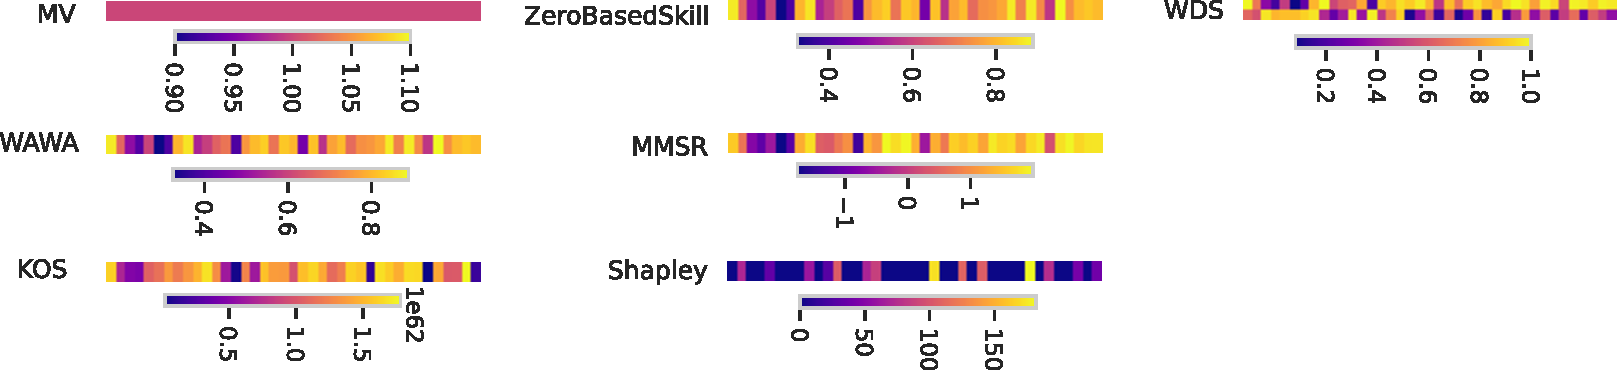
\includegraphics[width=\textwidth]{../matrix_weights_bluebirds_workers.pdf}
  \caption{Example of weights obtained for the BlueBirds dataset using the presented.}
  \label{fig:weights_by_strat}
\end{figure}

\section{Shapley label aggregation for crowdsourcing}
\label{sec:shapagg}

\subsection{Preliminaries on Shapley values}

Shapley values have been used to quantify the contribution of individual features in machine learning models' prediction \citep{molnar2020interpretable}.
In the context of crowdsourcing, we propose to use Shapley values to quantify the contribution of each worker to the final label aggregation.
We first recall the definition of a Shapley value.

\begin{definition}
Given a set of workers $T$ with $n_\text{worker}$, and a value function $\nu(\cdot): 2^T\rightarrow \mathbb{R}$ -- for example the prediction score of a classifier -- the Shapley value of a worker $j$ for a task $i$ is defined as the average marginal contribution of the worker $j$ to every subset of $T\setminus\{j\}$:
\begin{equation}
  \phi_j(i, T, \nu) = \sum_{S\subseteq T\setminus\{j\}} \frac{|S|!(n-|S|-1)!}{n!} \left[\nu(S\cup\{j\}) - \nu(S)\right]\enspace.
\end{equation}
When there is no ambiguity over the value function, we adopt the standard notation abuse $\phi_j(i, T, \nu)=\phi_j(i, T)$. Furthermore, if all workers participate then, $\phi_j(i, T)=\phi_j(i)$.
\end{definition}
Shapley values satisfy the following properties:
\begin{itemize}
  \item Symmetry: if $\nu(S\cup\{p\})=\nu(S\cup\{q\})$ for all set $S\subseteq T\setminus\{p,q\}$, then $\phi_p=\phi_q$.
  \item Null worker: if $\nu(S\cup\{p\})=\nu(S)$ for $S\subseteq [n_\text{worker}]$ then $\phi_p=0$.
  \item Additivity: for two value functions $\nu_1$ and $\nu_2$, $\phi_j(\nu_1+\nu_2)=\phi_j(\nu_1)+\phi_j(\nu_2)$.
  \item Efficiency: $\sum_{j=1}^{n_\text{worker}} \phi_j(\nu)=\nu(T)$.
\end{itemize}

Where the Shapley value is interesting for a crowdsourcing problem, is that if a worker does not help the classifier to predict the label, then its Shapley value will be close to zero. And, two workers with similar contributions will obtain similar Shapley values.

\subsection{Shapley label aggregation strategy}

We introduce the following label aggregation algorithm based on Shapley values.
It is based on the Expectation-Maximization procedure where we iteratively estimate the labels and the workers' skills until convergence -- \emph{e.g.} stabilization of the skills.
Given a current estimation of the labels and a classifier $\mathcal{C}$, we consider the skill of each worker as their total contribution in the predictions.
The contribution of a worker $j_0\in[n_\text{worker}]$ on a single task $i_0\in [n_\text{task}]$ is given as $|\phi_{j_0}(i_0)|\in\mathbb{R}_+$.

\begin{algorithm}[tbh]
  \caption{Shapley label aggregation strategy.}\label{alg:shap}
  \begin{algorithmic}[1]
    \State \textbf{Input:} classifier $\mathcal{C}$, $t_{\max}>0$ maximum number of iterations
  \State Initialize labels with MV: $\hat{y}_i^0 = \mathrm{WMV}(i, \mathbf{1}_{n_\text{worker}\times K})$ for each task $i\in [n_\text{task}]$
    \For{$t=0,\dots, t_{\max} - 1 $}
        \State Train classifier $\mathcal{C}$ on $\{(x_i, \hat{y}_i^t)_{i\in [n_\text{task}]}\}$
        \State Compute Shapley values' total contribution of each worker $j\in [n_\text{worker}]$:
        \[ \mathrm{contrib}(j) = \sum_{i=1}^{n_\text{task}} |\phi_{j}(i)|\enspace. \]
        \State Update weights: $W^t_{j,:} = \mathrm{contrib}(j)\mathbf{1}_K$ for each worker $j\in [n_\text{worker}]$
        \State Update labels with WMV: $\hat{y}_i^{t+1} = \mathrm{WMV}(i, W^{t})$ for $i\in[n_\text{task}]$.
    \EndFor
    \State \textbf{Output:} $\hat{y}_i^\text{shapley} = \hat{y_i}^{t_{\max}}$.
  \end{algorithmic}
  \end{algorithm}

First, note that in \Cref{alg:shap} the participation of each worker is linked to their total contribution. There is no upper bound on the skill estimation with $\mathrm{contrib}$ as we value a worker who answers multiple times.
However, if they answer many labels randomly, their Shapley value is close to zero and their total contribution is low.
As it can be seen in \Cref{fig:weights_by_strat}, as the Shapley values can be used for feature importance in prediction, it can also identify which workers are the most important for the final label aggregation and could be the center of more analysis.
And, at the same time, it can identify which workers are not contributing to the final label.

\subsection{Implementation}
\label{sub:implementation}

To compute Shapley values, we use the \texttt{Shap} library \citep{NIPS2017_7062}.
We use an XGBOOST classifier \citep{chen2016xgboost} as the classifier $\mathcal{C}$.
Shapleu values can thus be
Label aggregation strategies are implemented in Python using the \texttt{crowd-kit} \citep{CrowdKit2023} or \texttt{peerannot} \citep{peerannot} libraries.
The XGBOOST classifier is known to have an extensive number of hyperparameters to tune.
To choose them, we first use the \texttt{optuna} \citep{optuna} library to tune over a $3$-fold cross-validation of best hyperparameters for the set of tasks and label $\{(x_i, \hat{y}_i^0)_{i\in [n_\text{task}]}\}$.
This random search includes the trees' depth, learning rate, the number of trees, the minimum child weight, the subsampling proportion and regularizations. These best parameters are then used in \Cref{alg:shap} to iteratively train the XGBOOST model with the current label estimates.

\subsection{Evaluation metrics}

We evaluate the performance of the Shapley label aggregation strategy using the accuracy and the F1 score.
More precisely, each of the real datasets considered provides a -- partially known -- ground truth.
This test set is denoted $\mathcal{D}_\text{test}=\{(x_i, y_i^\star)\}_{i=1}^{n_\text{test}}$ and is used to evaluate the accuracy of the label aggregation strategies.
This ground truth is not used during the aggregation, only at evaluation time.
The accuracy of the aggregation strategy \texttt{agg} is the proportion of correctly predicted labels $(\hat[y]^\texttt{agg}_i)_{i=1}^{n_\text{test}}$ over the total number of tasks in $\mathcal{D}_\text{test}$ with ground truth in $y^\star=(y_i^\star)_{i=1}^{n_\text{test}}$:
\[\mathrm{Accuracy}(\hat{y}^\texttt{agg}, y^\star) = \frac{1}{n_\text{test}}\sum_{i=1}^{n_\text{test}} \mathds{1}(\hat{y}^\texttt{agg}_i=y_i^\star) \enspace.\]
We take into account the possible class imbalance by presenting a macro-average F1 score. Denoting respectively $\mathrm{TP}_k$, $\mathrm{FP}_k$ and $\mathrm{FN}_k$ the true positives, false positives and false negatives related to the class $k\in[K]$, the macro averaged F1-score writes
\[
\mathrm{F1} = \frac{1}{K}\sum_{k=1}^K\frac{\mathrm{TP}_k}{\mathrm{TP}_k + 0.5(\mathrm{FN}_k + \mathrm{FP}_k)}\enspace.
\]
This score is commonly used to evaluate the balance between precision and recall in classification tasks. It provides a measure of the quality of the label aggregation strategy when dealing with imbalanced datasets.

These metrics are evaluated on several real datasets.
The BlueBirds dataset \citep{WelinderEtal10b} is a binary classification ($K=2$) dataset with $n_\text{task}=108$ tasks and $n_\text{worker}=39$ workers.

\section{Results}
\label{sec:results}
\subsection{Performance on real datasets}

We evaluate the Shapley label aggregation strategy on several real datasets.
From \Cref{tab:scores}, we see that using Shapley-based weights in the WMV strategy outperforms other strategies in terms of accuracy and F1 score.
Note that the KOS strategy can not be applied to the datasets considered with $K>2$ as it is only suited for binary classification tasks.

\begin{table}[h]
  \centering
  \caption{Accuracy and F1 Score of the WMV-based label aggregation strategies over 4 real datasets.}
  \label{tab:scores}
  \footnotesize{
  \begin{tabular}{l|cc|cc|cc|cc}
  \hline
  \multirow{2}{*}{\textbf{Strategy}} & \multicolumn{2}{c|}{\textbf{BlueBirds}} & \multicolumn{2}{c|}{\textbf{Df 2}} & \multicolumn{2}{c|}{\textbf{Df 3}} & \multicolumn{2}{c}{\textbf{Df 4}} \\
  \cline{2-9}
   & \textbf{Accuracy} & \textbf{F1 Score} & \textbf{Accuracy} & \textbf{F1 Score} & \textbf{Accuracy} & \textbf{F1 Score} & \textbf{Accuracy} & \textbf{F1 Score} \\
  \hline
  MV    & 0.759 & 0.742 & 0. & 0. & 0. & 0. & 0. & 0. \\
  WAWA  & 0.759 & 0.742 & 0. & 0. & 0. & 0. & 0. & 0. \\
  ZBS   & 0.648 & 0.623 & 0. & 0. & 0. & 0. & 0. & 0. \\
  WDS   & 0.759 & 0.736 & 0. & 0. & 0. & 0. & 0. & 0. \\
  KOS   & 0.630 & 0.570 & 0. & 0. & 0. & 0. & 0. & 0. \\
  M-MSR & 0.639 & 0.578 & 0. & 0. & 0. & 0. & 0. & 0. \\
  \rowcolor{lightgray} Shapley & \textbf{0.805}& \textbf{0.794}& & & & & & \\

  \hline
  \end{tabular}
  }
  \end{table}
% \subsection{Performance varying the number of workers}

% From the real datasets, we can explore how the number of workers impacts the performance of the different label aggregation strategies.
% To do so, given a dataset, we randomly choose the same subset of $5$ workers for the label aggregation strategies.
% Then, we add workers one by one, chosen uniformly at random, and evaluate the accuracy and F1 score of the label aggregation strategies with the new set of workers.



\subsection{More information on workers}

\begin{figure}[htb]
  \centering
  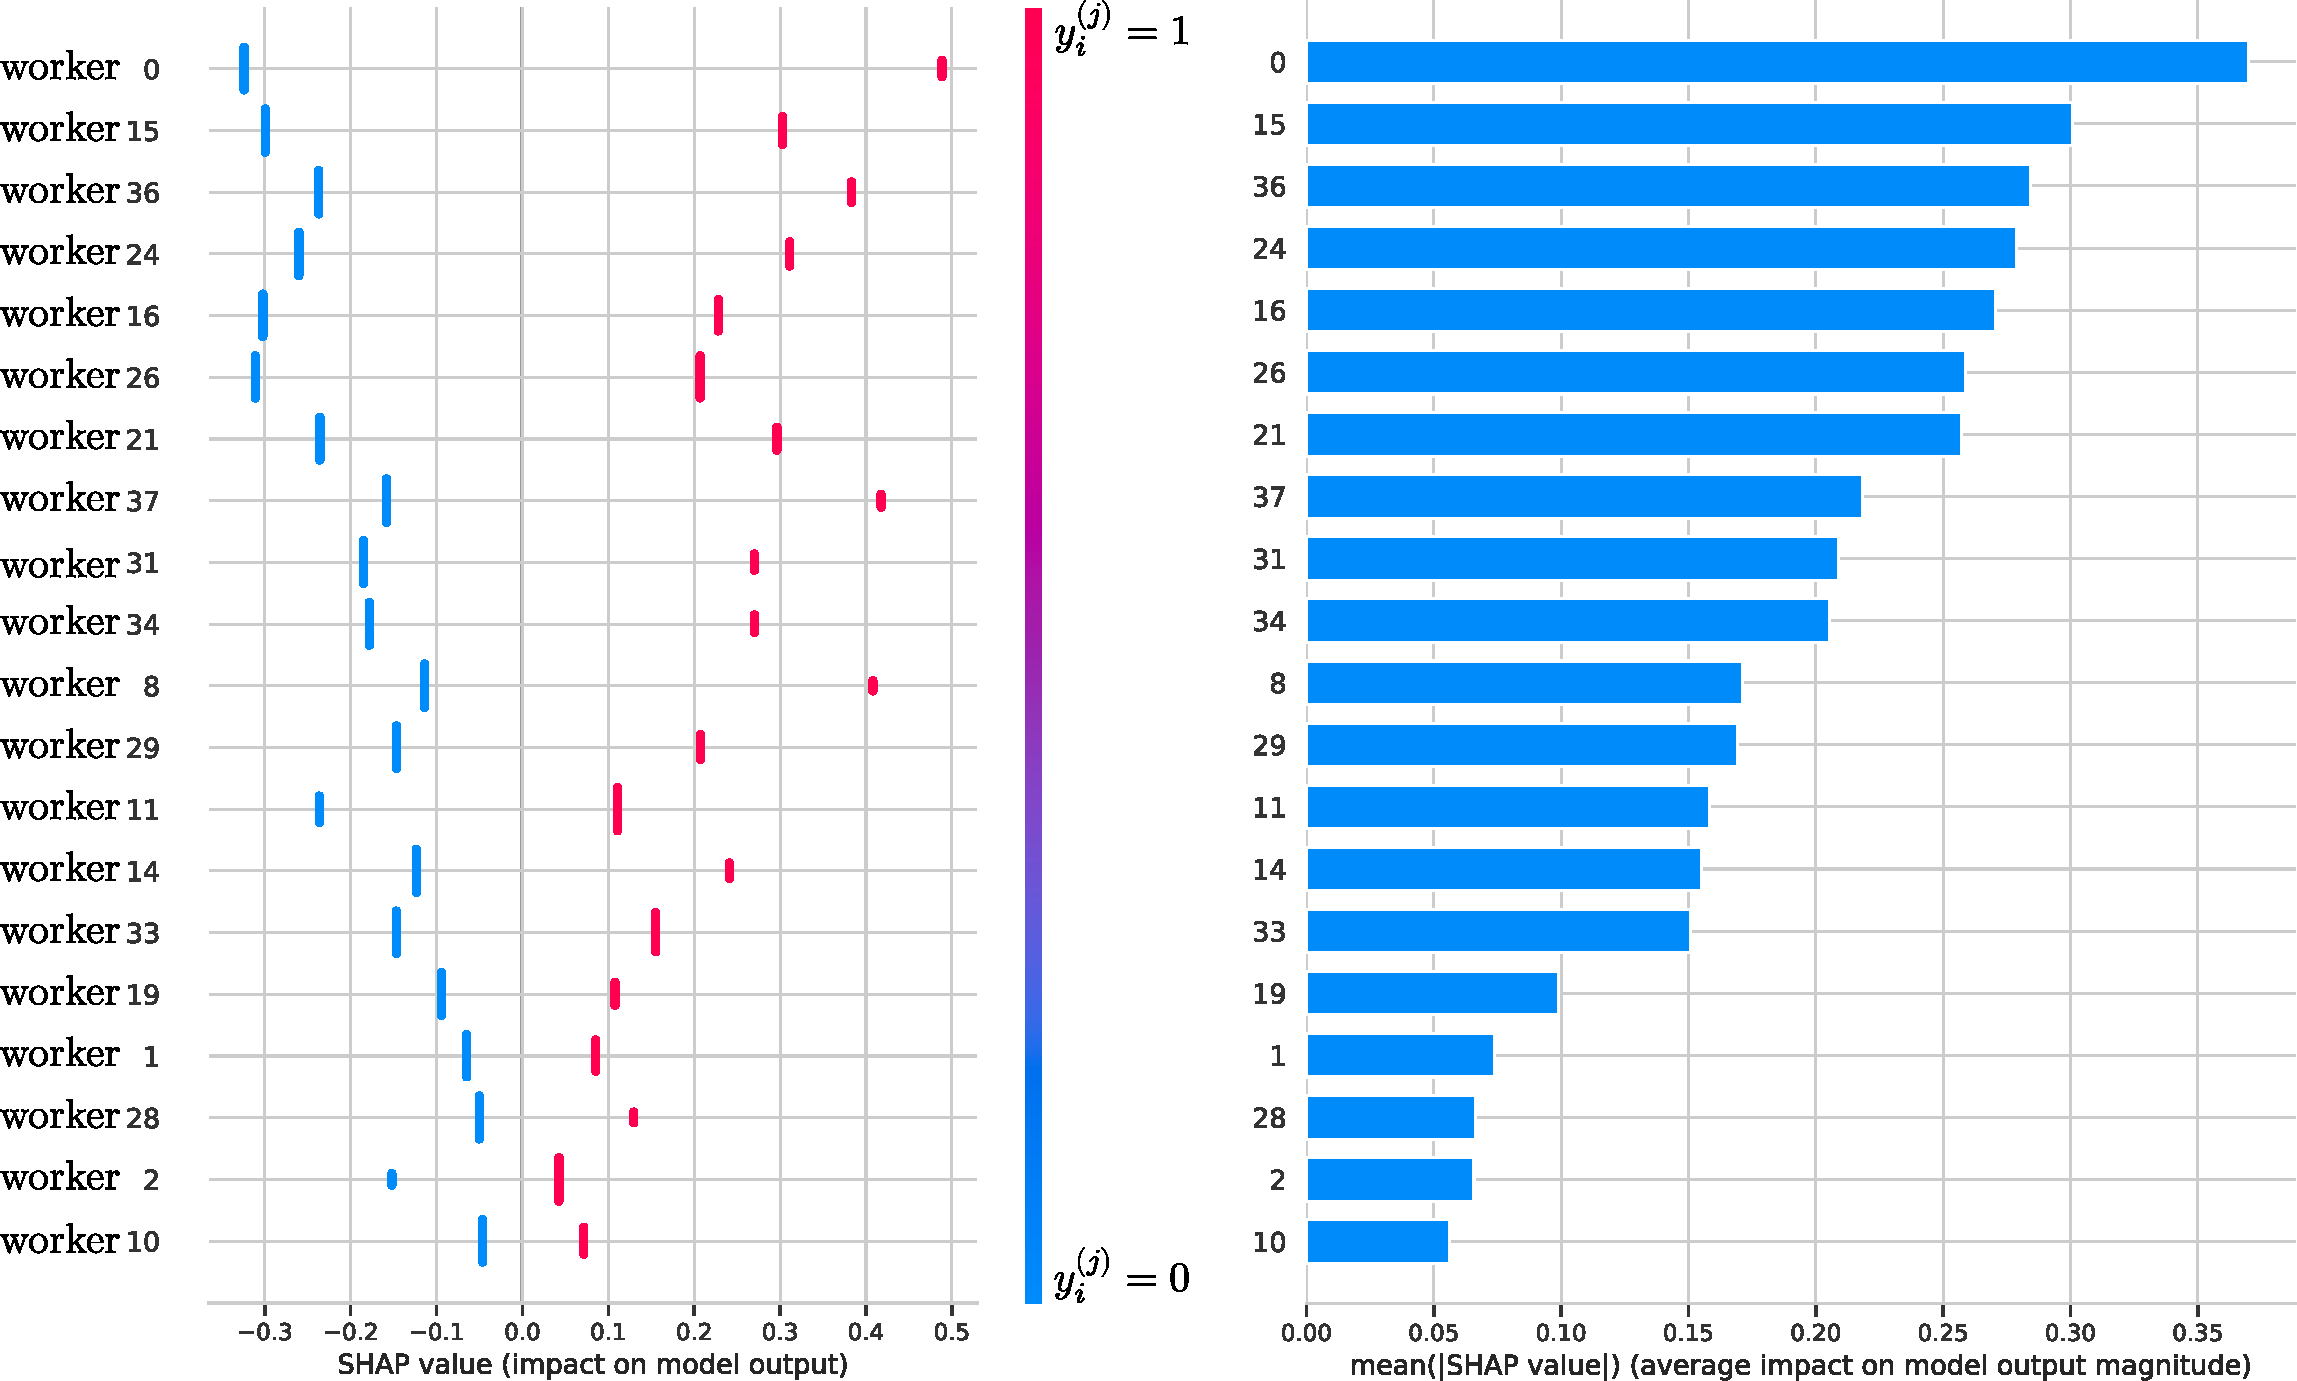
\includegraphics[width=\textwidth]{./../summary_plot_shap_all_bluebirds.pdf}
  \caption{Summary of the main contributing workers for the BlueBirds dataset using Shapley values. Left: Worker $0$ has the highest contribution to the final label -- either for class $0$ or $1$, followed by worker $15$. Then, worker $36$ has better identification for class $1$ than class $0$. Right: Average impact of each worker on the final predicted label by the XGBOOST classifier. This worker's contribution scalar value -- used in \Cref{alg:shap} weight $w(j, \cdot)$ -- does not allow to differentiate between classes.}
  \label{fig:shap_bluebirds}
\end{figure}

Using the Shapley values as workers' contribution, we can also provide more information on the workers' reliability.
Let us explore the BlueBirds' dataset Shapley weights as an example.
From \Cref{fig:shap_bluebirds}, we see that worker $0$ has the best overall contribution to the final label.
Note that this order of contribution given by Shapley values is in agreement with the accuracy of the workers even though Shapley values are not directly linked to the accuracy of a model.
Indeed, as we know the ground truth, we can compute the accuracy of each worker.
The accuracy of worker $0$ is $0.80$, worker $15$ is $0.73$ -- the two main workers contributing to the final aggregation -- and worker $10$ is $0.5$ (random answers).
The worker $22$ -- not represented in \Cref{fig:shap_bluebirds} as they are not a main contributor -- has an accuracy of $0.42$ -- worse than a random guess -- and an average absolute contribution of $0.03$ to the final label. This worker is indeed not contributing to the final label given the poor quality of their answers.

Worker $15$ is the second-best contributor, and worker $36$ has a better identification for class $1$ than class $0$.
However, as we use a single scalar value that is class-blind in \Cref{alg:shap} to aggregate the label in the WMV, this asymmetrical contribution is not taken into account.
This is a limitation of the current Shapley label aggregation strategy.


\section{Conclusion}
\label{sec:conclusion}

We introduced a new label aggregation strategy based on Shapley values for crowdsourcing classification tasks.
In the framework of weighted majority votes, we used the Shapley values as workers' weights to aggregate the labels.
We showed that this strategy outperforms other weighted majority vote strategies on real datasets in terms of accuracy and F1 score.
Moreover, we discussed how Shapley-based skills can be used to explore workers' reliability.
However, this strategy is limited by the scalar value used to aggregate the labels in the WMV strategy.
Not unlike most other WMV strategies, it does not take into account per-class skills.
An extension of this work would be to consider multidimensional skills based on Shapley values for each worker, allowing for a per-class contribution to the final label and a finer estimation of workers' skills.

\bibliographystyle{apalike}
\bibliography{cap2024}

\end{document}
